\documentclass[border=5pt]{standalone}
\usepackage{tikz}
\usetikzlibrary{calc, positioning}
\usepackage{amsmath}
\begin{document}
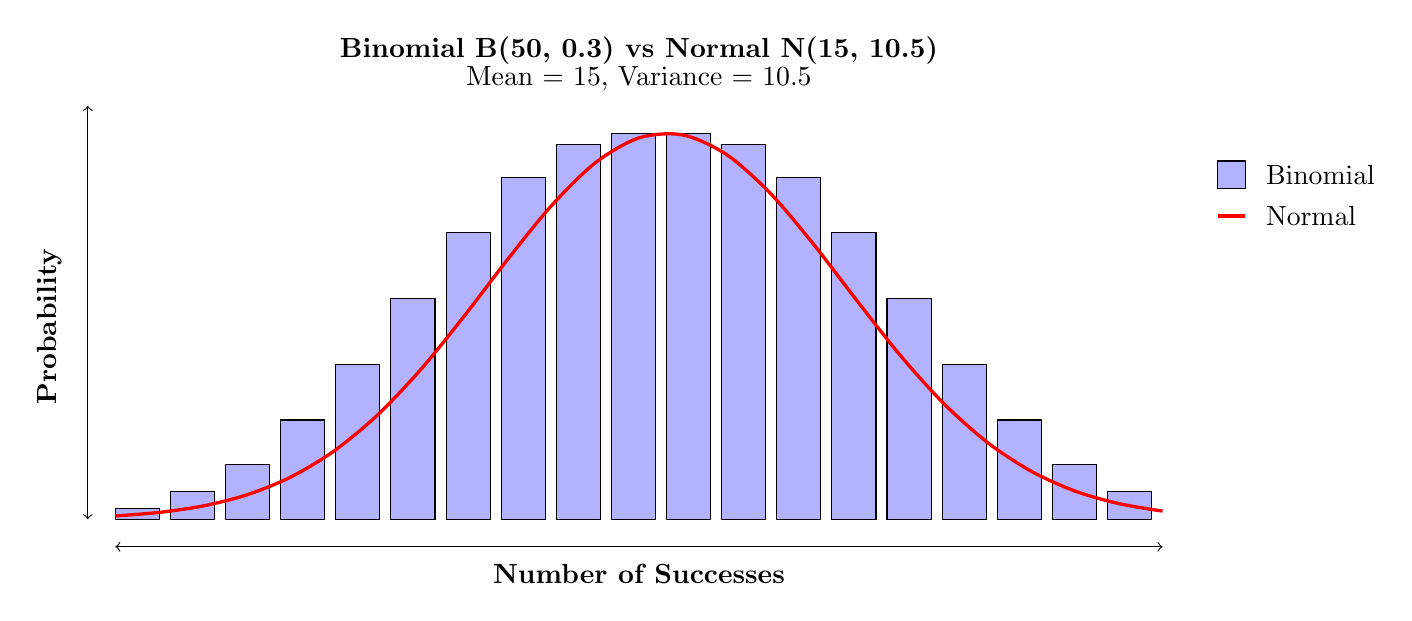
\begin{tikzpicture}[scale=0.7]
% Binomial histogram bars (manually calculated approximate values)
\draw[fill=blue!30, draw=black] (5, 0) rectangle (5.8, 0.2);
\draw[fill=blue!30, draw=black] (6, 0) rectangle (6.8, 0.5);
\draw[fill=blue!30, draw=black] (7, 0) rectangle (7.8, 1.0);
\draw[fill=blue!30, draw=black] (8, 0) rectangle (8.8, 1.8);
\draw[fill=blue!30, draw=black] (9, 0) rectangle (9.8, 2.8);
\draw[fill=blue!30, draw=black] (10, 0) rectangle (10.8, 4.0);
\draw[fill=blue!30, draw=black] (11, 0) rectangle (11.8, 5.2);
\draw[fill=blue!30, draw=black] (12, 0) rectangle (12.8, 6.2);
\draw[fill=blue!30, draw=black] (13, 0) rectangle (13.8, 6.8);
\draw[fill=blue!30, draw=black] (14, 0) rectangle (14.8, 7.0);
\draw[fill=blue!30, draw=black] (15, 0) rectangle (15.8, 7.0);
\draw[fill=blue!30, draw=black] (16, 0) rectangle (16.8, 6.8);
\draw[fill=blue!30, draw=black] (17, 0) rectangle (17.8, 6.2);
\draw[fill=blue!30, draw=black] (18, 0) rectangle (18.8, 5.2);
\draw[fill=blue!30, draw=black] (19, 0) rectangle (19.8, 4.0);
\draw[fill=blue!30, draw=black] (20, 0) rectangle (20.8, 2.8);
\draw[fill=blue!30, draw=black] (21, 0) rectangle (21.8, 1.8);
\draw[fill=blue!30, draw=black] (22, 0) rectangle (22.8, 1.0);
\draw[fill=blue!30, draw=black] (23, 0) rectangle (23.8, 0.5);

% Normal curve overlay N(15, 10.5)
\draw[red, very thick] plot[smooth, domain=5:24] (\x, {7*exp(-(\x-15)^2/(2*10.5))});

% Labels and annotations
\draw[<->] (5, -0.5) -- (24, -0.5);
\node at (14.5, -1) {\textbf{Number of Successes}};
\draw[<->] (4.5, 0) -- (4.5, 7.5);
\node[rotate=90] at (3.8, 3.5) {\textbf{Probability}};
\node at (14.5, 8.5) {\textbf{Binomial B(50, 0.3) vs Normal N(15, 10.5)}};
\node at (14.5, 8) {Mean = 15, Variance = 10.5};

% Legend
\draw[fill=blue!30, draw=black] (25, 6) rectangle (25.5, 6.5);
\node[right] at (25.7, 6.25) {Binomial};
\draw[red, very thick] (25, 5.5) -- (25.5, 5.5);
\node[right] at (25.7, 5.5) {Normal};
\end{tikzpicture}
\end{document}
